\documentclass[10pt,letterpaper]{article}
\usepackage[top=1in,bottom=1in,left=1in,right=1in]{geometry}
\usepackage{datetime}
\usepackage{natbib}      % http://merkel.zoneo.net/Latex/natbib.php
\usepackage{palatino}
\usepackage{verbatim}
\usepackage[normalem]{ulem}
\bibpunct{(}{)}{;}{a}{,}{,}

\usepackage{array}

\usepackage{chngpage}
\usepackage{stmaryrd}
\usepackage{amssymb}
\usepackage{amsmath}
\usepackage{graphicx}
\usepackage{lscape}
\usepackage{subfigure}
\usepackage[usenames,dvipsnames]{color}
\definecolor{myblue}{rgb}{0,0.1,0.6}
\definecolor{mygreen}{rgb}{0,0.3,0.1}
\usepackage[colorlinks=true,linkcolor=black,citecolor=mygreen,urlcolor=myblue]{hyperref}

\newcommand{\bocomment}[1]{\textcolor{Bittersweet}{BO says: #1}}

\newcommand{\ignore}[1]{}
\newcommand{\transpose}{^\mathsf{T}}
\newcommand{\inner}[1]{\langle #1 \rangle} 
\newcommand{\smallsec}[1]{\noindent \textbf{#1\ }}
\newcommand{\cmd}[1] {{\color{blue}\texttt{#1}}}
\newcommand{\norm}[1]{\left\lVert#1\right\rVert} % needs to be included for DIP notation!

\newcommand{\solution}[1]{{\color{myblue} \emph{[Solution:} 

#1 

\emph{End solution]}}}
\newcommand{\solutionnote}[1]{{\color{myblue} \emph{[Note:}

#1 

\emph{End note]}}}
\newcommand{\points}[1]{{\color{mygreen}\emph{[#1]\ \ }}}

\newcommand{\aone}{\diamondsuit}
\newcommand{\atwo}{\heartsuit}
\newcommand{\bone}{\triangle}
\newcommand{\btwo}{\Box}
\newcommand{\myand}{\ \land\ }
\newcommand{\myor}{\ \lor\ }
\newcommand{\mynot}{\lnot}

\title{
  \textbf{Mini-project 5} \\
  \Large{CMPSCI 670, Fall 2019, UMass Amherst} \\
  \Large{Instructor: Subhransu Maji} \\
  \Large{TAs: Aruni RoyChowdhury, Archan Ray}
}

\settimeformat{ampmtime}
\date{}
\begin{document}
\maketitle

\renewcommand\thesubsection{\thesection.\alph{subsection}}


\section*{Guidelines}

\paragraph{Submission.} Submit a \emph{single pdf document} via moodle that includes your solutions, figures and code. The latex source file for the homework is provided which you can modify to produce your report. You are welcome to use other typesetting software as long as the final output is a pdf. For readability you may attach the code printouts at the end of the solutions within the same pdf. Note that we will not run your code. Similarly figures should be included in a manner which makes it easy to compare various approaches. Poorly written or formatted reports will make it harder for the TA to evaluate it and may lead to a partial deduction of credit. 

\paragraph{Late policy.} You could have 24 hours late submission with a 50\% mark down. Late submission beyond 24 hours will not be given \emph{any} credits.

\paragraph{Plagiarism.} We might reuse problem set questions from previous years, covered by papers and webpages, we expect the students not to copy, refer to, or look at the solutions in preparing their answers. We expect students to want to learn and not google for answers. 

\paragraph{Collaboration.} The homework must be done individually, except where otherwise noted in the assignments. 'Individually' means each student must hand in their own answers, and each student must write their own code in the programming part of the assignment. It is acceptable, however, for students to collaborate in figuring out answers and helping each other solve the problems. We will be assuming that you will be taking the responsibility to make sure you personally understand the solution to any work arising from such a collaboration.

\paragraph{Using other programming languages.} We made the starter code available in Python and Matlab. You are free to use other languages such as Octave or Julia with the caveat that we won't be able to answer or debug non Matlab/Python questions.

\paragraph{Python requirements.} We will be using Python 2.7. The Python starter code requires \cmd{scipy}, \cmd{numpy} (at least v1.12), and \cmd{scikit-image}.
If you are not familiar with installing those libraries through some package manager (like \cmd{pip}), the easiest way of using them is installing \href{https://docs.anaconda.com/anaconda/install/}{Anaconda}.




\newpage


\section*{The MNIST dataset}
In this part your goal is to implement several image
features and evaluate their performance using logistic-regression classifiers and
convolutional networks on three variants of the MNIST digits dataset:

\begin{itemize}
\item \textbf{normal} -- the standard MNIST dataset (File \cmd{digits-normal.mat})
\item \textbf{scaled} -- where the pixel values of each image in the normal dataset are replaced as $I \leftarrow a*I + b$ where $a$ and $b$ are random numbers $\in [0,1]$ (File \cmd{digits-scaled.mat}). 
\item \textbf{jittered} -- where the image is translated within each image randomly between $[-10,10]$ pixels both in the horizontal and vertical directions (File \cmd{digits-jittered.mat}).
\end{itemize}

The ``normal" dataset can be loaded into Matlab by typing $\cmd{load('../data/digits-normal.mat')}$. 
In Python, we added a function in \cmd{utils.py} called \cmd{loadmat} that does the same thing. 
This loads a structure called \cmd{data} which has the images, labels and the splits in variables \cmd{x}, \cmd{y}, and \cmd{set} respectively. 
E.g., $\cmd{data.x}$ is an array of size $28 \times 28 \times 1 \times2000$ containing $2000$ digits. 
Class labels are given by the variable $\cmd{data.y} \in \{0,1,\ldots, 9\}$. 
Thus, pixel \cmd{(i,j)} in the the \cmd{k'th} training example is \cmd{data.x(i,j,1,k)} with label \cmd{data.y(k)}. 
The \cmd{data.set} has values $\in\{1,2,3\}$ corresponding to train, val, and test splits respectively.
In Python, \cmd{data} is a dictionary and you can access the fields in a similar way:
\cmd{data.y} is \cmd{data['y']}, \cmd{data.set} is \cmd{data['set']}.
An important difference is that \cmd{data['x']} is an array of size $28 \times 28 \times 2000$ instead of $28 \times 28 \times 1 \times2000$.
So, the pixel \cmd{(i,j)} in the the \cmd{k'th} training example is \cmd{data['x'][i,j,k-1]} with label \cmd{data['y'][k-1]}.

\begin{figure}[h]
\centering
\begin{tabular}{ccc}
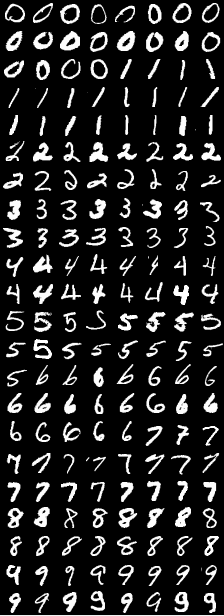
\includegraphics[width=0.25\linewidth]{digits-normal.png} & 
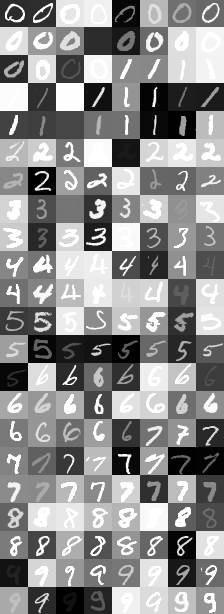
\includegraphics[width=0.25\linewidth]{digits-scaled.png} & 
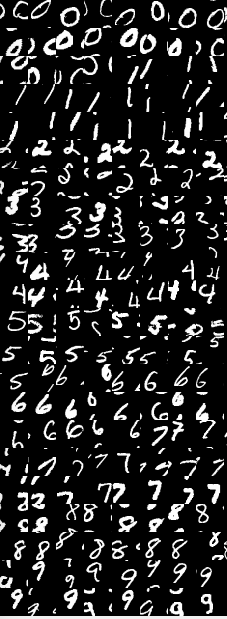
\includegraphics[width=0.25\linewidth]{digits-jittered.png} \\
(a) normal & (b) scaled & (c) jittered \\
\end{tabular}
\caption{Example images from different variants of the MNIST
  dataset. You can visualize the images using $\cmd{montageDigits}$
  function included in the codebase.} 
\end{figure}


\newpage

\section{Handcrafting image representations}

Implement three different image representations described below. 

\begin{enumerate}

\item \textbf{Pixel features.}  Implement the function \cmd{features = extractDigitFeatures(x, 'pixel')} that takes as input the images \cmd{x} and returns their pixel values as a feature. You have to simply reshape the $28\times28$ pixel image into a vector of size $784\times 1$. The variable \cmd{features} is a array of size $784\times N$ where $N$ is the number of images in \cmd{x}. 

\item \textbf{Histogram of oriented gradients.}
Implement the function \cmd{features = extractDigitFeatures(x, 'hog')} that takes as input the images \cmd{x} and returns their histogram of oriented gradients (HoG) as a feature. Recall the steps in the HOG feature computation are:
\begin{enumerate}

\item Apply non-linear mapping to the values of the image. In the HOG paper of Dalal and Triggs, CVPR 2005, mapping the pixel intensities through a non-linearity such as $x \leftarrow x^{\gamma}$ or $x \leftarrow \log(x)$ was found to be useful.

\item Compute horizontal and vertical gradients $g_x$ and $g_y$ at each pixel using derivative operators. Compute the magnitude $m = \sqrt{g_x^2 + g_y^2}$ and orientation $\theta=\arctan(g_y/g_x)$ at each pixel. Note that this version of angle lies between $-\pi/2$ to $\pi/2$. You may also use the version that computes angles between $-\pi$ to $\pi$ using $\theta=\arctan(g_x, g_y)$. Construct the orientation bins accordingly.
\item Given a \cmd{binSize} and number of orientations (\cmd{numOri}) define a grid of \cmd{binSize} $\times$ \cmd{binSize} pixels across the image. Within each cell compute the orientation histogram by assigning each pixel to the nearest orientation in \cmd{numOri} and with vote proportional to the gradient magnitude. Concatenate these histograms to obtain an image representation. Use a spatial binSize of 4 and 8 orientation bins.
\item Local and global feature normalization. 

\end{enumerate}

To begin with you can ignore initial non-linear mapping (Step 1) and
local normalization (Step 4). You will investigate the effect of
global normalization as described in the next section.

\item \textbf{Local binary patterns.} In class we discussed various
  ways of constructing a bag-of-words representation for images. The
  steps are (1) extract local features on a dense grid or at
  interest points, (2) assign them to codewords based on a learned
  dictionary,  and (3) build a histogram of word counts per
  image. Local binary patterns (LBP) combine feature extraction and
  codeword assignment and have been shown to be
  highly effective for image classification.

  Your goal is to implement a simplified version of LBP in this homework. In
this version you will represent each image as a collection of all of
its 3x3 patches (overlapping). If each pixel is represented by a 8 bit
intensity value then the number of such patches are $8^{(3\times
  3)}=134,217,728$, which is far larger than the number of pixels in
an image. Clustering these patches across images would give you a
dictionary. 


The LBP approach instead directly maps each 3x3 patch into a number
between 0 and 255 as follows. Consider the pixels in a 3x3
patch. Subtract from each pixel the value of the center pixel and assign
them a bit value of 1 if the value of the pixel is greater than zero,
and a bit value of 0 otherwise. This gives us a 8-bit representation (excluding the
center which is always 0) of every 3x3 patch. Thus each 3x3 patch can
be represented by a integer between 0-255. The scheme is shown in the
Figure~\ref{fig:lbp}.


\begin{figure}[h]
\centering
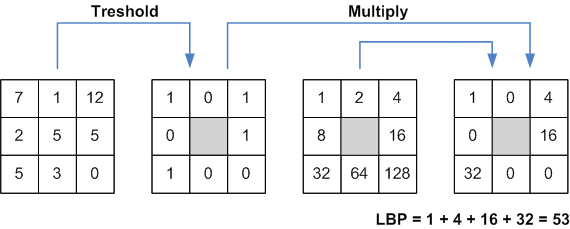
\includegraphics[width=0.5\linewidth]{lbp.png}
\caption{\label{fig:lbp} Illustration of the LBP feature computation for a 3x3 patch.} 
\end{figure}

To obtain an image representation apply this scheme to each 3x3 patch
in the image and obtain a histogram that indicates how many patches
get mapped to each integer. Implement the function \cmd{features =
  extractDigitFeatures(x, 'lbp')} that takes as input the images
\cmd{x} and returns a local binary pattern (LBP) histogram for each
image. This feature should be 256 dimensional.
\end{enumerate}

\subsection{Feature normalization}

After you implement these features you may find that the scales of the
features vary across images. For example, on the ``scaled"
version of the dataset the images exhibit varying contrast levels
making pixel representations less robust. 
Feature normalization can alleviate some of these issues and improve
classification performance with simple machine learning models. 

Your goal is to implement the following normalization steps:

\begin{enumerate}
\item \textbf{Square-root scaling} -- replace the value of each feature by its square-root, i.e., $x \leftarrow \sqrt{x}$.

\item \textbf{L2-normalization} -- scale each feature vector to unit length in Euclidean sense, i.e., if $\mathbf{x}$ is a vector then the L2-normalized version would be $\mathbf{x} \leftarrow \mathbf{x}/\sqrt{\sum_i \mathbf{x}_i^2}$.
\end{enumerate}

The effectiveness of one or both of these steps depends on the dataset and feature types.

\section{Multiclass logistic regression}
In multiclass logistic regression with K classes the predicted probability of class k for input $\mathbf{x}$ is given by:
\begin{equation}
\hat{y}^{(k)} = P(Y = k|X = x) = \frac{\exp(\mathbf{w}_k^T\mathbf{x})}{\sum_{i=1}^K \exp(\mathbf{w}_i^T\mathbf{x})}, 
\end{equation}
where ${\mathbf{w}_1, \mathbf{w}_2, \ldots, \mathbf{w}_k}$ are the model parameters.
Training minimizes the cross-entropy loss over the training set $\{(\mathbf{x}_i, y_i)\}$ plus a regularization term to encourage simpler models given by
\begin{equation}
\min_{\mathbf{w}_1, ..., \mathbf{w}_K} L = \min_{\mathbf{w}_1, \mathbf{w}_2, \ldots, \mathbf{w}_k} \sum_i \ell (y_i, \hat{y}_i) + \lambda \sum_k ||\mathbf{w}_k||^2_2, 
\end{equation}

where $\hat{y}_i = P(Y|X=x_i)$ and $\ell(y, \hat{y})$ is the cross-entropy loss

\begin{equation}
\ell (y, \hat{y}) = -\sum_{k=1}^{K} y^{(k)} \log \hat{y}^{(k)}.
\end{equation}

While there is no closed form solution to minimize the objective we
can still find the solution with gradient descent. Derive the
expression for the $i^{th}$
component in the vector gradient of $L$ with respect to $\mathbf{w}_k$
and write down the update rule for $\mathbf{w}_k$ using $\eta$ for the
step size. 
Note that in class we discussed the online and batch
version of the gradient. This dataset is small enough that batch
gradients can be computed.



Implement the logistic-regression classifier inside the function \cmd{model = trainModel(x, y)}, which in turn calls the function \cmd{model = multiclassLRTrain(x, y, param)}. The \cmd{multiclassLRTrain} method runs batch gradients using a fixed learning rate for a given number of iterations to compute the model parameters. You might have to adjust these hyperparamters (eta, lambda, maxiter) to obtain good performance across feature types.

Similarly implement the function \cmd{ypred = multiclassLRPredict(model,x)} that computes predictions for new data points.

One important note is that you may find adding a bias term to the end of the features can be helpful. You can accomplish this by simply adding a constant feature to the end of the all the feature vectors. Don't forget to account for this at test time. For this task you will find that running gradient descent with a fixed learning rate for a large number of iterations finds good model parameters. This shouldn't be surprising since the objective is convex.

\subsection{Training, cross-validation, testing}

The entry code for the homework is in the file \cmd{testMNIST}. It loops over different  variants of the dataset, calls the function \cmd{extractDigitFeatures} for three different feature types $\in$ \{'pixel', 'hog', 'lbp'\}, trains a logistic-regression model on the training set and evaluates the model on the validation set. The function 
\cmd{[acc, conf] = evaluateLabels(y, ypred, false)} returns the accuracy and confusion matrix (\cmd{conf}) given the true labels \cmd{y}, and predictions \cmd{ypred}. When the last parameter is \cmd{true} it additionally displays the confusion matrix. You may find this helpful for intermediate debugging.

Currently the \cmd{extractDigitFeatures} simply returns zero features for all methods  and all methods perform at 10\% accuracy on all datasets which is the chance performance. You will implement your approach here. Each training step has several hyperparameters, such as normalization method, size of bin for oriented gradient features, as well as classifier-specific ones such as learning rates, regularization term. These should be tuned on the validation set (\cmd{testSet=2}). Once you have found the optimal values, you can change the \cmd{testSet=3} to evaluate the method on the test set.

The confusion matrix ($c$) is a 10x10 array where the $c(i,j)$ entry counts how many times a class $i$ got classified as class $j$. A perfect classifier should have all non-zero values in the diagonal. You can use this to visualize which pair of classes get confused most by different features.


\section{Convolutional neural nets}
Investigate a convolutional neural network (CNN) for these tasks using a library of your choice. 
Your starting point will be architectures that consists of several convolutional and pooling layers, followed by a one or more linear layers similar to the LeNet architecture discussed in class. 
Your goal is to compare CNNs to handcrafted representations on the provided datasets. 
Most deep learning libraries provide example code for MNIST classification using CNNs. 
Perhaps the simplest way is to convert the datasets provided in the codebase to a format readable by the library to get started. Links to popular deep learning frameworks are linked below.

Note that the dataset in the homework is \emph{different} from the standard MNIST dataset that comes with example code in various packages. 
Make sure you modify the code and load the provided dataset instead. 
If you are working in Python, you may find scipy.io.loadmat() useful for loading data from mat files.
Since our dataset is relatively small and the training models with many parameters can lead to over-fitting. Therefore, you may want to experiment with shallower CNNs with a few convolutional, pooling, non-linearity blocks, followed by a linear layer or two for predicting class labels.

Explore a few different architecture choices and hyperparamters such as learning rates, weight decay (regularization term) on the validation set and report the result on the test set.


\subsection{Software packages}
PyTorch and TensorFlow are two popular deep learning frameworks based on python, while MatConvNet is a popular one for on Matlab. Feel free to use any of these for this part of the homework, or any other package that you are familiar with. Here are links to some of these frameworks:
\begin{itemize}
\item \textbf{TensorFlow.} Tutorials: \url{https://www.tensorflow.org/tutorials}
\item \textbf{PyTorch.} Tutorial: \url{http://pytorch.org/tutorials/beginner/deep_learning_60min_blitz.html}
MNIST example: \url{https://github.com/pytorch/examples/blob/master/mnist/main.py}.
\item \textbf{MatConvNet.} 
Example: \url{https://github.com/vlfeat/matconvnet/tree/master/examples/mnist}. 
Tutorial: \url{http://www.vlfeat.org/matconvnet/training/}
\end{itemize}

% \newpage

\section{Answer the following questions [70 points]}
\begin{enumerate}
\item \points{10 points} Implement the multi-class logistic regression training and evaluation. Include the gradient update equation for the parameters in your writeup and attach the code for training and evaluation at the end.
\item \points{5 points} Describe your experiments using pixel features and logistic regression. In particular you should:
\begin{itemize}
\item Report the accuracy on the validation and test set.
\item Describe what normalization steps were effective on what datasets.
\item Include the values of hyperparameters that worked best on the validation set.
\end{itemize}
\item \points{15 points} Answer all the above questions for HoG
  features. Don't forget to include the hyperparameters specific to
  HoG features such as numOri and binSize.
\item \points{15 points} Answer all the above questions for LBP features.
\item \points{20 points} Answer all the above questions for CNN. In particular note what architectures you tried.
\item \points{5 points} Which feature worked the best on each version of the
  dataset? Briefly explain your answer.

\end{enumerate}

In your submission include your implementation of \cmd{extractDigitFeatures}. As a reference my implementation of various features with suitable normalization obtains the following accuracy on the validation set. With careful cross-validation you may be able to outperform these numbers.

\begin{verbatim}
      +++ Accuracy Table [trainSet=1, testSet=2]
      -------------------------------------
      dataset           pixel hog   lbp	
      -------------------------------------
      digits-normal.mat	87.00	82.00	74.00	
      digits-scaled.mat	77.40	79.00	74.00	
      digits-jitter.mat	20.40	34.00	71.60	
\end{verbatim}

With some modifications of the LeNet architecture the CNN can reach about 95\%, 90\%, 70\% accuracy on normal, scaled and jittered set respectively. 
Training CNNs takes longer so plan accordingly. 
As a rough estimate, a network with two convolutional layers and one fully-connected layer took about 30 minutes to train on a laptop CPU.
Most libraries can take advantage of GPU hardware if your machine has any. That could speed up your training times by a factor of 10 or more.

While we don't expect you to match these results exactly, if your numbers that are significantly off  might suggest a bug in the code. If that happens, we expect you to investigate why that's the case.

\newpage

\section{Image denoising with deep image priors [30 points]}

Given a noisy image $x_0$ we can find its denoised version $x^*$ through the following minimization:
\begin{equation}
x^* = \min_x E(x, x_0) + P(x)
\end{equation}
where $E(x, x_0)$ is a \emph{data term} that measures how close is $x$ to $x_0$ and $P(x)$ is the \emph{prior term}.
This formulation can be interpreted as a \emph{maximum a posteriori} (MAP) inference in a Bayesian setting.
However, defining a good prior $P(x)$ for natural images is challenging. 
In class we discussed a Gaussian mixture model over patches as an example, but the resulting minimization and learning is challenging. 
We also discussed procedural priors such as Gaussian smoothing, median filtering, and non-local means, which you implemented in Mini-project 2. 
In this part we will investigate convolutional networks as image priors.


\href{https://arxiv.org/abs/1711.10925}{Recent research} shows that convolutional networks for image generation can be effectively used to induce a prior over natural images (aka ``deep image prior").
The main idea is that instead of searching over images $x$ in the optimization, we look for images that can be generated through a convolutional neural network of a fixed architecture on a fixed input.
It turns out that random convolutional networks produce ``smooth" images and encode natural image priors. 
We will exploit this strategy for denoising images, by changing the network parameters different to produce the target (noisy) images starting from a random initialization.


Let the network be $f_\theta(\eta)$ where $\theta$ are parameters of the network and $\eta$ is an  input. The input is sampled from a standard Gaussian distribution and kept fixed.
Now, we can denoise $x_0$ as follows:

\begin{align}
\label{eq:dip}
\theta^* = \min_\theta E(f_\theta(\eta), x_0); \qquad x^* = f_{\theta^*}(\eta).
\end{align}

The error for denoising is the squared distance between the pixels, i.e., $ E(f_\theta(\eta), x_0) = \norm{f_\theta(\eta) - x_0}_2^2$.
Notice that there is no prior term and the objective can simply be minimized by gradient descent.


A question remains about which architecture we should use for $f_\theta$.
A good starting point is the following, but feel free to come up with other variations.
We will employ a fully-convolutional encoder-decoder architecture with 6 convolutional layers.
The first 3 are correspond to the encoder part of the network.
It consists of 3 $\texttt{ConvBlocks}$, which are built using a 2D-convolution (with stride$=2$) with several 3$\times$3 filters, followed by batch normalization and ReLU activation.
The last 3 layers are $\texttt{DeconvBlocks}$, built by using a bilinear upsampling followed by a 2D-convolution (with stride=1), batch normalization and ReLU activation.
With this architecture the output size is the same as the input. In this case the input is simply a random image (each pixel is drawn from a zero mean Gaussian or Uniform distribution) of the same size as the target image.
Batch normalization speeds up training significantly.
Once again feel free to use any software package you like to implement these layers. For example, PyTorch, TensorFlow, and MatConvNet provide implementations of these layers.


Fitting a neural network to a single image poses a huge risk of over fitting. You will find running gradient descent for a long time will cause the training error to go to zero resulting in no denoising!To avoid this can you can stop the optimization early. 

For this question we will use the images provided in the \cmd{data/denoising} folder which contains:
\begin{itemize}
\item \texttt{saturn.png, saturn-noisy.png, lena.png, lena-noisy.png}
\end{itemize}
The first image pair will be familiar to you from Mini-project 2, but this version is slightly resized.
Gaussian noise was added to create the noisy versions for both cases.
As a reference Gaussian filtering and Median filtering produce the following results on the two images (see the enclosed \cmd{evalDenoisingBaseline.m}.)

\begin{figure}[h]
\centering
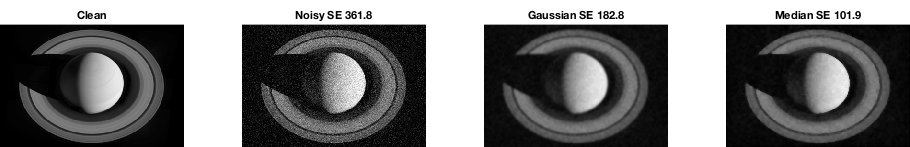
\includegraphics[width=0.95\linewidth]{saturn-output.png}
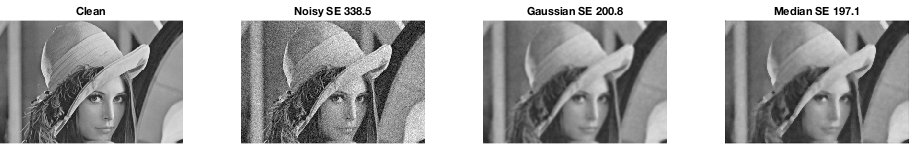
\includegraphics[width=0.95\linewidth]{lena-output.png}
\caption{\label{fig:bayer} Image denoising with Gaussian and Median filter.}
\end{figure}


\subsection{Implementing the deep image prior}

We have provided a python-based skeleton for the deep image prior in \cmd{evalDenoising} script, which uses the PyTorch library. 
The \cmd{evalDenoising} script loads the clean and the noisy image, visualizes them, and computes the error (squared-distance) between them.
It then initializes a convolutional network (you will implement this) and runs several iterations of gradient descent.
Your goal is to denoise the images using the deep image prior, which
should result in a lower error value. With careful architecture design
and early stopping you should be able to reduce the noise level
significantly.

\begin{itemize}
\item \points{20 points} \textbf{Network architecture and random
  image.} The first step is to implement the architecture described
  before. You will use the following number of filters for each layer:
  16, 32, 64. The kernel size of each filter is 3$\times$3.	
The decoding part of the architecture is simply a mirrored
version. Once the architecture is implemented, you will execute
\cmd{evalDenoising}, which will instantiate your network, sample a
random input $\eta$ and show the image generated by the random
architecture. In Python, you will implement your network in the file
\cmd{dip.py}. Show five images generated by the network in your report
by sampling different random inputs and network parameters.

\item \points{6 points} \textbf{Using the deep image prior.}
  In this step you will use the network you created in the
  previous step to minimize Equation~\ref{eq:dip}. You will
  use squared error as a data-term ($E(x,y) =
  \norm{x-y}_2^2$). Run 500 gradient steps using Adam
  optimizer with learning rate$=0.01$. Report the results for
  both the images as well as the error with respect to the
  reference. Also plot the training and testing error as a
  function of the number of iterations.

  \emph{Tip: Start with a shallower network, say with just one or two
    encoder-decoder layers, to debug your code.}
\item \points{4 points} Run gradient descent for 5000 iterations. Are
  the images generated after 5000 iterations better than the ones
  generated after 500 iterations? Why?

\end{itemize}

As a reference 500 iterations of gradient descent takes 3 minutes on my laptop.

\subsection{Extensions [Extra 10 points]}
Here are some suggestions for extra credit. You can implement one of these:

\begin{itemize}
\item \textbf{Improving the results.} Take a look at the original
  paper \url{https://arxiv.org/abs/1711.10925} and explore different
  strategies to improve the results. For example deeper architectures,
  those with skip connections, as well as averaging the results across
  iterations. Also take a look at this paper that characterizes why
  the deep image prior works \url{https://arxiv.org/abs/1904.07457}.


\item \textbf{Image demosaicing with deep image prior.} Come up with a data-term in the loss function that can be used instead of the squared error in order to perform image demosacing with the deep image prior. Run your algorithm on the images from Mini-project 2 and compare them to the baselines.
\end{itemize}


\section{Report Writing and Conclusion [10 points]}
As usual, please follow the guidelines for writing a good report to earn points for writing and presentation. We request that you do not share your solutions publicly or privately.
Making these took quite a bit of effort and we would like to reuse them in the future.

Finally, congratulations on finishing all mini projects. Hope it was fun and have a cake!
\begin{figure}[h]
\centering
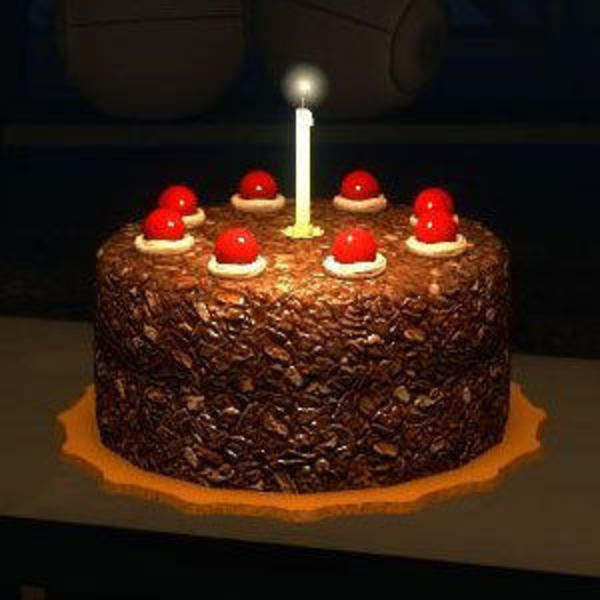
\includegraphics[width=1in]{portal-cake.jpg}
\end{figure}
\end{document}
